\documentclass{article}
\usepackage{amsmath}
\usepackage{subcaption}
\usepackage{mathtools}
\usepackage{graphicx}
\usepackage{epstopdf}
\DeclarePairedDelimiter\floor{\lfloor}{\rfloor}
\title{BrainGames PCA+STFT}
\begin{document}
\maketitle
Due to the limitation of the Muse Headband, we are limited to 5 channels. Therefore, the raw data matrix will only have 5 “features”.
  \begin{align}
    raw\:data &= \begin{bmatrix}
            x_{11} & x_{12} & x_{13} & \dots  & x_{15} \\
   		   x_{21} & x_{22} & x_{23} & \dots  & x_{25} \\
            \vdots & \vdots & \vdots & \ddots & \vdots \\
            x_{m1} & x_{m2} & x_{m3} & \dots  & x_{m5}
         \end{bmatrix}
  \end{align}
However, directly applying PCA to these 5 features has been proven ineffective. There are 2 major reasons for that. \\
\\
1. The feature set is already small enough, there is really no point to reduce it further\\
2. The data in each channel/feature is sinusoidal in nature, therefore the direction that would maximize the variance of any channel is simply the direction of the time, which does not yield any useful data partitions\\
\\
-----------------------------------------------------------------------------------------------------\\
Therefore, the goal of this document is to provide the correct procedure to use PCA with sinusoidal EEG data. Let us start out by defining some useful data vectors and constraints.\\
\\
A representative channel demonstrates the biggest visual difference in EEG graph when the subject switched tasks.\\
\begin{figure}
  \begin{subfigure}[b]{0.5\textwidth}
    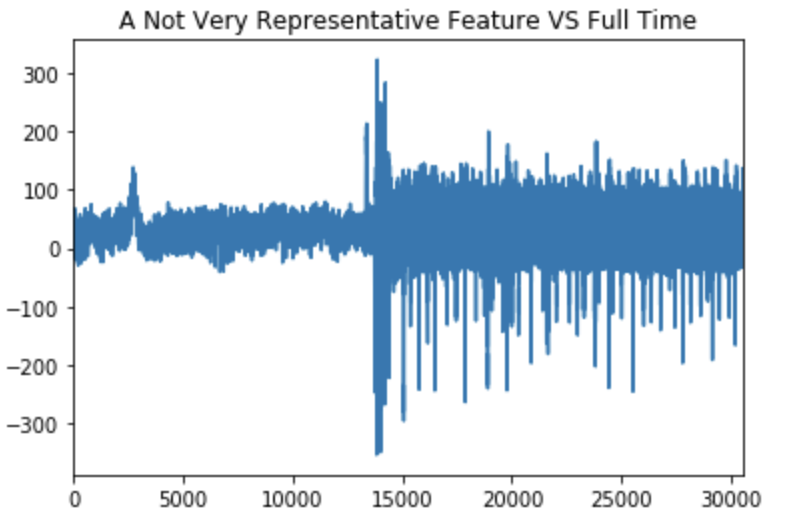
\includegraphics[width=\textwidth]{norepr}
    \label{fig:1}
  \end{subfigure}
  %
  \begin{subfigure}[b]{0.5\textwidth}
    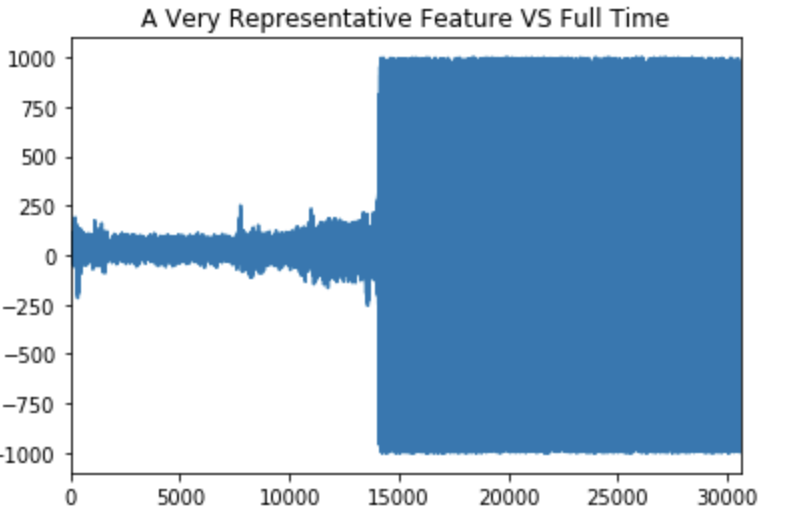
\includegraphics[width=\textwidth]{repr}
    \label{fig:2}
  \end{subfigure}
\end{figure}

   \begin{align}
   	representative\:channel &= \begin{bmatrix}
            x_{1} \\
            x_{2} \\
            \vdots \\
            x_{m}
         \end{bmatrix}
   \end{align}
   \begin{align}
   	m &= number\: of\: data\: points \\
   	T &= duration \:of \:the \:data \:collection (seconds) \\
   	t &= duration\: of \:each\: window (seconds)\\
   	w &= numbe\:r of\: windows = T/t\\
   	dpw &= number\: of\: data\: points \:per \:window = m/w\\
   	r &= residual \:data = m \:(mod \:dpw)\\
   	N &= the \:closest \:power\: of\: 2\: to\: dpw
   \end{align}
You prune the representative channel by deleting floordiv(r,2) elements from the top of the representative channel and ceildiv(r,2) elements from the bottom.
   \begin{align}
	pruned\:channel &= \begin{bmatrix}
            x_{1} \\
            x_{2} \\
            \vdots \\
            x_{w * dpw}
         \end{bmatrix}    
   \end{align}
Although this channel generated the most representative data, this data set only has one feature. In order to perform PCA effectively, we need to expand the feature set. Conveniently, Short Time Fourier Transform (STFT) solves this problem. STFT not only expands our feature set, it is also much better than the canonical DFT because STFT can deal with the transient and changing nature of the EEG signal. 
Intuitively, think of STFT as sliding a window across the 1-D data set and performs DFT along the way.
STFT performs DFT in an iterative procedure, each time moving through half of each window size that we previously defined. Essentially, if there are w windows, then you would run 2*w + 1 DFT ( STFT stops when its sliding window is completely disjoint with the data set) .
Applying STFT to the pruned data, we can get a new data matrix with more features and less data points.
\begin{align}
    new\:data &= \begin{bmatrix}
            x_{11} & x_{12} & x_{13} & \dots  & x_{1N} \\
   		   x_{21} & x_{22} & x_{23} & \dots  & x_{2N} \\
            \vdots & \vdots & \vdots & \ddots & \vdots \\
            x_{(2w+1)1} & x_{(2w+1)2} & x_{(2w+1)3} & \dots  & x_{(2w+1)N}
         \end{bmatrix}
  \end{align}
Each row of the new data matrix is the DFT result performed by the STFT sliding process. The problem is that each DFT result is complex valued, which is incompatible with PCA. Therefore, in order to perform PCA correctly, we need a little bit more knowledge on DFT, especially on what does a DFT result entails.

Let's start from the beginning, and keep one thing in mind: DFT is only invented because it gives a nice linear algebra view and also allowing a more convenient visual understanding of FFT. However, originally the big question is “How do we approximate a piece of sampled signal with a finite number of sinusoidals?”
We know that in the correct inner product space, signals can be represented by the sinusoidal basis, and here is the truncated approximation of a signal. 

Note: x(t) stands for the actual sampled signal in time domain, and X[i] stands for the coefficients/weight for each harmonics in frequency domain
   \begin{equation}
   	x(t)=\sum_{i=0}^{N-1} X_{i} e^{j2 \pi f_{0} i t}
   \end{equation} 
We will shortly prove that we can link DFT to this truncated representation of the signal. We first see that 
   \begin{equation}
   	e^{j2 \pi f_{0}  t} = e^{j2 \pi t / N} = {\omega^{t}}
   \end{equation} 
therefore, we can observe a pattern when we write down the sum with specific t,
 \begin{equation}
   	x(0) = \sum_{i=0}^{N-1} X_{i}  {{\omega^{0}}^{i}} 
   \end{equation} 
   \begin{equation}
   	x(1) = \sum_{i=0}^{N-1} X_{i}  {{\omega^{1}}^{i}}
   \end{equation} 
    \begin{equation}
   	x(2) = \sum_{i=0}^{N-1} X_{i}   {{\omega^{2}}^{i}} 
   \end{equation} 
We observe that this is essentially a matrix-vector product between the DFT matrix and X
\begin{equation}
DFT = \frac{1}{\sqrt{N}}\left[\begin{array}{cccccc}{1} & {1} & {1} & {1} & {\cdots} & {1} \\ {1} & {\omega} & {\omega^{2}} & {\omega^{3}} & {\cdots} & {\omega^{N-1}} \\ {1} & {\omega^{2}} & {\omega^{4}} & {\omega^{6}} & {\cdots} & {\omega^{2(N-1)}} \\ {1} & {\omega^{3}} & {\omega^{6}} & {\omega^{9}} & {\cdots} & {\omega^{3(N-1)}} \\ {\vdots} & {\vdots} & {\vdots} & {\vdots} & {\ddots} & {\vdots} \\ {1} & {\omega^{N-1}} & {\omega^{2(N-1)}} & {\omega^{3(N-1)}} & {\cdots} & {\omega^{(N-1)(N-1)}}\end{array}\right]
\end{equation}
\begin{align}
   	signal\: x &= \begin{bmatrix}
            x_{1} \\
            x_{2} \\
            \vdots \\
            x_{N}
         \end{bmatrix}
\end{align}
\begin{align}
   	weights\: of\: harmonics\: X &= \begin{bmatrix}
            X_{1} \\
            X_{2} \\
            \vdots \\
            X_{N}
         \end{bmatrix}
\end{align}

We have the following relationship:
\begin{equation}
   	x = DFT * X
   \end{equation} 
We observe that x is a real vector, but X contains complex numbers, how do we justify this discrepancy? We need to apply the complex-conjugate-symmetry property of DFT, which is proven below.
\begin{equation}
X^{*}[N-k]=X^{*}[-k]=\left(\sum_{t=0}^{N-1} x[t] e^{-j 2 \pi f_{0}(-k) t}\right)^{*}
\end{equation}
\begin{equation}
=\sum_{n=0}^{N-1} x[n] e^{-\left(-j 2 \pi(-k) \frac{n}{N}\right)} = X[k]
\end{equation}
From this property, we can immediately tell X[0] and X[N/2] are guaranteed to be real, but how about the other elements? Let us assume that X[k] = a+bj and X[N-k] = a-bj.
Then in the summation of the truncated Fourier Series, we show that X[k] terms and X[N-k] terms will sum to a real number, which would make the entire sum real.
\begin{equation}
(a+bj)\left(e^{j 2 \pi f_{0}(k) t}\right) = (a+b j)\left(\cos (2 \pi f_{0} k t)+j \sin \left(2 \pi f_{0} k t\right)\right)
\end{equation}
\begin{equation}
(a-bj)\left(e^{j 2 \pi f_{0}(-k) t}\right) = (a-b j)\left(\cos (2 \pi f_{0} (-k) t)+j \sin \left(2 \pi f_{0} (-k )t\right)\right)
\end{equation}
Eq.26 can be rewritten as 
\begin{equation}
(a-bj)\left(e^{j 2 \pi f_{0}(-k) t}\right) = (a-b j)\left(\cos (2 \pi f_{0} k t)-j \sin \left(2 \pi f_{0} kt\right)\right)
\end{equation}
Adding Eq.25 and Eq.27, the sum becomes
\begin{equation}
2a\left(\cos (2 \pi f_{0} k t)\right) - 2b\left(sin (2 \pi f_{0} kt)\right)
\end{equation}
So we update each row of the new data matrix. Instead of using the complex coefficients, we replace them with the real coefficients a, b. Now we can perform PCA on this set of real data points. And since we aren't doing PCA in the time domain (sinusoidal) but rather in the frequency domain, we are essentially trying to characterize EEG signal based on the weights of its harmonics since the data points spread along the different directions of harmonics rather than a single axis where the sinusoidal wave propagates, and this is a much more indicative understanding of the EEG signal decomposition.

[ View toy example at: https://github.com/lytzV/BrainGames ]
\end{document}